\begin{figure}
	\centering
	\begin{subfigure}[b]{0.45\textwidth}
		\centering
		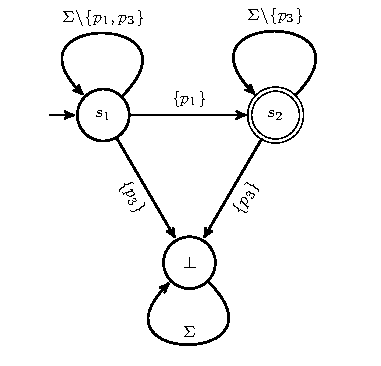
\includegraphics[width=\textwidth]{images/example_1_graph}
		\caption{$\bot\Release(\neg p_3\vee p_1\vee p_2) \wedge \top\mathcal{U}p_1$}
		\label{fig:g1}
	\end{subfigure}
	\hfill
	\begin{subfigure}[b]{0.45\textwidth}
		\centering
		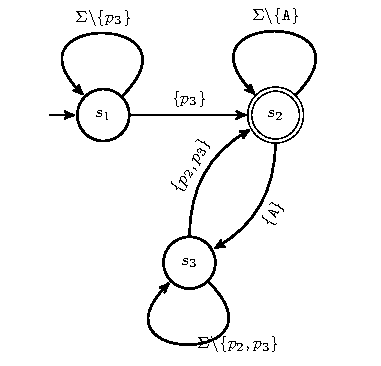
\includegraphics[width=\textwidth]{images/example_2_graph}
		\caption{$\bot\Release(\neg\texttt{A}\vee(\top\Until(p_2\vee p_3)))\wedge\top\Until p_3$}
		\label{fig:g2}
	\end{subfigure}
	\caption{Representation of LTL$_f$ formulae as constraint automaton from \cite{LeoniMA12,Westergaard11}.}
	\label{fig:g1g2}
\end{figure}

\section{Working Assumptions}\label{sec:wa}
In this section, we outline some working assumptions that can be inferred from the literature of reference. First, we assume that we only want to deal with log traces \cite{XuLZ17a}; this implies that \begin{enumerate*}[label=\emph{\alph*})] \item the semantics of the Declare models can be expressed in Linear Time Logic on Finite Traces (LTL$_f$) \cite{10.1007/978-3-642-40176-3_8}, as logs are finite sets of finite traces \cite{GiacomoV13}; \item we work under the closed world assumptions, as the only possible set of traces that might satisfy a Declare constraints might come from its associated constraint automaton and, possibly, from the set of log traces; \item differently from \cite{MultiPerspective}, we can avoid to model reading and writing operation, as the entirety of our analyses will be conducted \textit{post-mortem}; \item last, each event trace must be represented by one single proposition \cite{XuLZ17a}. \end{enumerate*} The latter consideration will require us to partition the possible data space into distinct propositions. Still, we can freely assume that the constraint automatons generated from the LTL$_f$ interpretation of such Declare constraints allow to represent any possible event label that is not represented within the Declare constraints, by either representing it as a transition $\Sigma\backslash S$, where $\Sigma$ is the set of all the possible strings and $S$ is a (possibly empty) finite set of traces that we want to ignore \cite{LeoniMA12,Westergaard11}, or by representing it as a predicate $\bigwedge_{i\leq n} \neg p_i$ \cite{Lydia}, where $p_1\dots p_n$ are all the possible propositions that can be deduced from a Declare Model represented in LTL$_f$. Figure~\ref{fig:g1g2} provides a intuitive representation of some LTL$_f$ formulae in the former representation.

We assume that all the data-aware predicate for the Declare clauses are always expressed in propositional calculus, where the atomic predicates are always in the form ``$\texttt{A}.\textit{var}\;\Re\; c$'', where \texttt{A} is a trace label containing a property named \textit{var} which is put in a binary relation $\Re$ with a constant value $c$, representing either a number or a string: e.g., $\Re$ could be either an equality or a precedence/subsequent relation or their negation. This is a widely adopted assumption, that spans from data-aware procedural models \cite{MultiPerspective} to data-aware declarative models \cite{10.1007/978-3-642-40176-3_8}. Furthermore, this assumption can be also adapted to categorical data, as strings are ordered via lexicographical orderings over the single characters \cite{MultiPerspective}.

Last, we freely assume that all the events having the same label will always contain the same set of keys, with possibly differently associated values. This is a common assumption in relational database field, where all the rows belonging to the same table contain the same number of values. We also freely assume that missing values are represented with specific values, such as an empty string, $0$, $-\infty$, or $+\infty$, depending on the context.